\chapter{\label{cha:sts_introduction}Introduction to Semantic Textual Similarity}

Semantic Textual Similarity (STS) measures the equivalence of meanings between two textual segments. In Natural Language Processing (NLP), measuring the semantic similarity between two textual segments plays an important role. It is a fundamental task for many NLP applications and their related areas. To measure STS, the input will always be two textual segments, and the output will be a continuous value representing the degree of similarity between the two input textual segments \autocite{agirre-etal-2012-semeval}. These segments can be short snippets of texts, complete sentences or even documents \autocite{agirre-etal-2013-sem}.

STS is related to both textual entailment (TE) and paraphrasing but differs in several ways. TE is the task of identifying the relationship between two texts commonly addressed as text (t) and hypothesis (h). Entailment, contradiction, and neutral are the most popular relationship types in TE \autocite{10.1007/11736790_9,marelli-etal-2014-semeval}. On the other hand, paraphrasing identification is the task of recognising text fragments with approximately the same meaning within a specific context \autocite{info11050241}. Therefore, TE and paraphrasing give a categorical output while STS identifies the degree of equivalence between two texts as a continuous value. 

Measuring STS is an important research problem, having many applications in NLP such as information retrieval (IR) \autocite{10.1145/1097047.1097051, 5571521}, text summarisation \autocite{ALIGULIYEV20097764, SCHALLEHN2004361}, question answering \autocite{mohler-etal-2011-learning}, relevance feedback \autocite{WANG2020102342}, text classification \autocite{10.1007/978-3-642-41278-3_74, 10.1007/978-3-319-11749-2_8} and word sense disambiguation \autocite{10.1007/978-3-642-17432-2_44}. In the field of databases, text similarity can be used for schema matching. In the document databases like Elasticsearch\footnote{Elasticsearch is a document database based on the Lucene library. It is available on \url{https://www.elastic.co/}. More information on the Similarity module is available on \url{https://www.elastic.co/guide/en/elasticsearch/reference/current/index-modules-similarity.html}}, there is a core module called \textit{"Similarity module"} that defines the document matching process. Furthermore, STS is also useful for relational join operations in databases where join attributes are textually similar to each other \autocite{10.1145/352595.352598, SCHALLEHN2004361}. STS is also widely used in semantic web applications such as community extraction \autocite{10.1007/978-3-642-14589-6_33}, Twitter search \autocite{feng-etal-2013-twitter} where the ability to measure semantic relatedness between concepts or entities accurately is required.
 
These applications need to measure STS automatically, which means that computer programs are necessary to calculate the STS between two textual inputs. The most natural way to approach this problem is to use a machine learning approach where the computer learns from examples. The development of rule-based methods would be too cumbersome, and would be unlikely to lead to robust solutions. Over the years, researchers have proposed numerous ML solutions for STS. These ML solutions can be categorised into two main categories; 
 \begin{enumerate*}[label=(\alph*)]
 	\item Linguistic feature-based and,
 	\item Vector/ Embedding-based.
 \end{enumerate*}
Most of the early approaches belong to the linguistic feature-based category. With this, features for the ML algorithm were hand-crafted. Such features include edge-distances between nodes in WordNet \autocite{10.1145/219717.219748}, number of named entities in two input texts, corpus pattern analysis features etc. These features would be then fed into an ML algorithm such as Support Vector Machine (SVM), Linear Regression etc. \autocite{bechara-etal-2015-miniexperts}. This ML algorithm will be trained on an annotated STS dataset and can then be used to measure STS automatically. Despite being extremely popular before the neural network era, linguistic feature-based algorithms have limitations. Determining the best linguistic features for calculating STS is not an easy task as it requires a good understanding of the linguistic phenomenon and relies on researchers' intuition. In addition, most of these features depend on lexical knowledge bases, such as WordNet, which makes it difficult to adopt them in to languages other than English. Furthermore, these features primarily rely on parsers that are not available in other languages \autocite{2016IJCA}. However, these methods' most significant limitation would be that they no longer provide strong results compared to the vector-based methods \autocite{cer-etal-2017-semeval}. 

With the introduction of word embeddings \autocite{DBLP:journals/corr/abs-1301-3781}, ML solutions in NLP shifted from feature-based methods to vector-based methods. Pre-trained word embedding models such as Word2vec \autocite{DBLP:journals/corr/abs-1301-3781}, GloVe \autocite{pennington-etal-2014-glove} and  fastText \autocite{mikolov-etal-2018-advances} provide a learned representation for texts where the words with the same meaning have a similar representation. Since these word embeddings are already semantically powerful, ML solutions no longer need to depend on lexical knowledge bases. As a result, embedding based ML solutions are easy to adapt for different languages as long as the pre-trained embeddings are available in that language. Furthermore, these solutions are now state-of-the-art in NLP tasks, including STS, providing stronger results than feature-based ML solutions \autocite{cer-etal-2017-semeval}. Therefore, as STS solutions in this part of the thesis,  we mainly explore embedding based ML approaches.

Similarly to general ML algorithms, vector-based ML STS algorithms can also be classified into two main categories; Supervised and Unsupervised. In supervised learning, ML models will be trained using labelled data. Therefore, supervised ML algorithms require data that has already been annotated manually with the closest answer. On the other hand, for unsupervised learning, you do not need an annotated dataset. Unsupervised ML approaches would discover the features by themselves. Given that annotated STS data is not commonly available in many languages and domains, exploring both supervised and unsupervised STS methods is essential. Therefore, the first two chapters in this part of the thesis explore unsupervised STS methods, while the last two chapters explore supervised STS methods. 

The most common unsupervised STS approaches are vector aggregation methods like Word Vector Averaging, Word Mover's Distance \autocite{10.5555/3045118.3045221} and Smooth Inverse Frequency \autocite{DBLP:conf/iclr/AroraLM17}. In Chapter \ref{cha:sts_state_of_the_art_methods}, we explore them in detail. We identify the best vector aggregation method empirically by analysing them in different STS datasets. Finally, we propose a new state-of-the-art vector aggregation method based on contextual word embeddings that outperforms other methods. 

In Chapter \ref{cha:sts_sentence_encoders}, we explore another unsupervised STS method using sentence encoders. Sentence encoders are different from vector aggregation methods as they use end-to-end models to get sentence embeddings rather than using a simple aggregation method. They provide strong results compared to other unsupervised STS methods. We use three different sentence encoders and analyse their performance in various aspects of English STS and also evaluate their portability to different languages and domains. 


In Chapters \ref{cha:sts_siamese_neural_networks} and \ref{cha:sts_transformers}, we explore the most popular supervised STS approaches. Usually, in supervised vector-based STS approaches, word embeddings would be fed into a neural network like tree-structured neural networks \autocite{tai-etal-2015-improved} and Siamese neural networks \autocite{Mueller_Thyagarajan_2016}. Among them, Siamese neural networks have been widely used in STS and have additional advantages compared to other structures. Therefore, we discuss them comprehensively in Chapter \ref{cha:sts_siamese_neural_networks}. We evaluate the existing Siamese Neural Network architectures in STS datasets and propose a novel Siamese Neural Network architecture for smaller STS datasets that outperforms current state-of-the-art Siamese neural models.  We also assess its performance in different languages and domains.

In the final chapter of Part I of this thesis, we explore the newly released transformers in STS tasks. Transformers have taken the NLP field by storm, providing very successful results in various NLP tasks. In Chapter \ref{cha:sts_transformers}, we bring together various transformer architectures \autocite{devlin-etal-2019-bert,yang2019xlnet,liu2019roberta} and investigate their performance in various STS datasets. We explore the strengths and weaknesses of transformer models in regard to accuracy and efficiency and discover the possible solutions for their limitations.


The main contributions of this part of the thesis are as follows.

\begin{enumerate}
	\item Each chapter analyses using various supervised and unsupervised techniques to compute semantic textual similarity, benefiting a wide range of NLP applications. We empirically evaluate all of them in three English datasets, two non-English datasets and an out of domain dataset to explore their adaptability.  
	
	\item We propose a novel unsupervised STS method based on contextual word embeddings that outperforms current state-of-the-art unsupervised vector aggregation STS methods in all the English datasets, non-English datasets, and datasets in other domains.
	
	\item We propose a novel Siamese neural network architecture that is efficient and outperforms current state-of-the-art Siamese neural network architectures in smaller STS datasets. 
	
	\item We provide important resources to the community. The code of each chapter as an open-source GitHub repository and the pre-trained STS models will be freely available to the community. The link to the GitHub repository and the models will be discussed in the introductory section of each chapter. 
\end{enumerate}

The remainder of this chapter is structured as follows. Section \ref{sec:sts_intro_datsets} discusses the various datasets we used in the \textit{"Semantic Textual Similarity"} part of the thesis and briefly analyses the datasets for common properties. In Section \ref{sec:sts_evaluation}, we discuss the main evaluation metrics we used in the \textit{"Semantic Textual Similarity"} part of the thesis. The chapter finishes with our conclusions.


\section{Datasets}
\label{sec:sts_intro_datsets}
The popularity of STS is partially attributed to the large number of shared tasks organised in SemEval from 2012-2017 \autocite{agirre-etal-2012-semeval,agirre-etal-2013-sem,agirre-etal-2014-semeval,agirre-etal-2015-semeval,agirre-etal-2016-semeval,cer-etal-2017-semeval}. Firstly, they provided annotated datasets that can train STS ML models and evaluate them. Secondly, at the end of each shared task, the solutions submitted by the participants are published, and the best solutions can be considered as state-of-the-art STS methods. 

To maintain the versatility of our methods, we experimented with several English STS datasets as well as several non-English datasets and a dataset from a different domain, which we will discuss later in this section. These datasets carry different and interesting characteristics. Therefore, with the introduction, we also do an exploratory analysis of the dataset focussing on its various properties. All of the datasets which are described here are publicly available and can be considered as STS benchmarks. 

\subsection{English Datasets}
\begin{enumerate}
  \item \textbf{SICK dataset}\footnote{The SICK dataset is available to download at \url{https://wiki.cimec.unitn.it/tiki-index.php?page=CLIC}} - The SICK dataset contains 9927 sentence pairs with a 5,000/4,927 training/test split which were employed in the \textit{SemEval 2014 Task1: Evaluation of Compositional Distributional Semantic Models on Full Sentences through Semantic Relatedness and Textual Entailment} \autocite{marelli-etal-2014-semeval}. The dataset has two types of annotations: Semantic Relatedness and Textual Entailment. We only use the Semantic Relatedness annotations in our research. SICK was built based on two existing datasets: the 8K ImageFlickr dataset \autocite{rashtchian-etal-2010-collecting}\footnote{The 8K ImageFlickr data set is available at \url{http://hockenmaier.cs.illinois.edu/8k-pictures.html}}  and the SemEval-2012 STS MSR-Video Descriptions dataset \autocite{agirre-etal-2012-semeval}\footnote{The SemEval-2012 STS MSR-Video Descriptions dataset is available at \url{https://www.cs.york.ac.uk/semeval-2012/task6/index.html}}. The 8K ImageFlickr dataset is a dataset of images, where each image is associated with five descriptions. To derive SICK sentence pairs, the organisers randomly selected 750 images and sampled two descriptions from each of them. The SemEval2012 STS MSR-Video Descriptions data set is a collection of sentence pairs sampled from the short video snippets which compose the Microsoft Research Video Description Corpus\footnote{The Microsoft Research Video Description Corpus is available to download at \url{https://research.microsoft.com/en-us/downloads/38cf15fd-b8df-477e-a4e4-a4680caa75af/}}. A subset of 750 sentence pairs has been randomly chosen from this data set to be used in SICK. 
  
  To generate SICK data from the 1,500 sentence pairs taken from the source data sets, a 3-step process has been applied to each sentence pair, namely \textit{(i) normalisation, (ii) expansion and (iii) pairing} \autocite{marelli-etal-2014-semeval}. The \textit{normalisation} step has been carried out on the original sentences to exclude or simplify instances that contained lexical, syntactic or semantic phenomena such as named entities, dates, numbers, multiword expressions etc. In the \textit{expansion} step, syntactic and lexical transformations with predictable effects have been applied to each normalised sentence, to obtain \textit{(i)} a sentence with a similar meaning, \textit{(ii)} a sentence with a logically contradictory or at least highly contrasting meaning, and \textit{(iii)} a sentence that contains most of the same lexical items, but has a different meaning. Finally, in the \textit{pairing} step, each normalised sentence in the pair has been combined with all of the sentences resulting from the expansion phase and with the other normalised sentence from the pair. Furthermore, several pairs composed of completely unrelated sentences have been added to the data set by randomly taking two sentences from two different pairs \autocite{marelli-etal-2014-semeval}. 
  
  Each pair in the SICK dataset has been annotated to mark the degree to which the two sentence meanings are related (on a 5-point scale). The ratings have been collected through a large crowdsourcing study, where ten different annotators have evaluated each pair. Once all of the annotations were collected, the relatedness gold score was computed for each pair as the average of the ten ratings assigned by the annotators \autocite{marelli-etal-2014-semeval}. Table \ref{tab:sickdata} shows examples of sentence pairs with different degrees of semantic relatedness; gold relatedness scores are expressed on a 5-point rating scale. Given a test sentence pair, the machine learning models need to predict a value between 0-5, which reflects the relatedness of the given sentence pair. 
  
  \begin{table}[ht!]
  	\centering 	
  	\begin{tabular}{l|c} 
  		\hline
  		\multicolumn{1}{c|}{\textbf{Sentence Pair}} & 
  		\multicolumn{1}{c}{\textbf{Relatedness}}  \\
  		\hline
  		\makecell[l]
  		{1. A little girl is looking at a woman in costume. \\ 
  		 2. A young girl is looking at a woman in costume.} & 4.7  \\
  		\hline
  			\makecell[l]
  		{1. Nobody is pouring ingredients into a pot. \\ 
  			2. Someone is pouring ingredients into a pot. } & 3.5  \\
  		\hline
  		\makecell[l]
  		{1. Someone is pouring ingredients into a pot. \\ 
  		 2. A man is removing vegetables from a pot. } & 2.8  \\
  		\hline
  		\makecell[l]
  		{1. A man is jumping into an empty pool. \\ 
  		 2. There is no biker jumping in the air. } & 1.6  \\
  		\hline               
  	\end{tabular}
  	\caption[Example sentence pairs from the SICK dataset]{Example sentence pairs from the SICK dataset with their gold relatedness scores (on a 5-point rating scale). \textbf{Sentence Pair} column shows the two sentence and \textbf{Relatedness} column denotes the annotated relatedness score.}
  	\label{tab:sickdata}
  \end{table}

Figure \ref{fig:sick_relatedness} shows the distribution of the relatedness value in the SICK training and SICK test sets. It is clear that there are more sentence pairs with high relatedness values compared to low relatedness values. The SICK training and SICK test follow similar distributions. 


\begin{figure}
	\captionsetup[subfigure]{justification=centering}
	\centering
	\begin{subfigure}[b]{.5\textwidth}
		\centering
		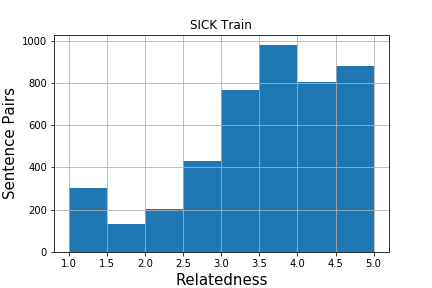
\includegraphics[width=\textwidth]{figures/semantic_textual_similarity/introduction/sick_train_relatedness_hist.png}
		\caption{Relatedness distribution of \\ SICK training test}
		\label{fig:sick_train_relatedness}
	\end{subfigure}%
	\begin{subfigure}[b]{.5\textwidth}
		\centering
		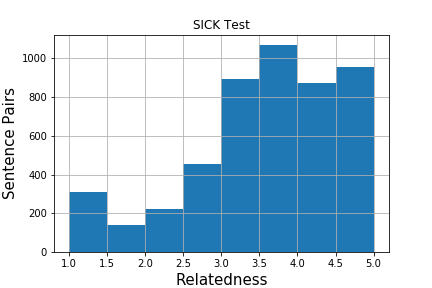
\includegraphics[width=\textwidth]{figures/semantic_textual_similarity/introduction/sick_test_relatedness_hist.png}
		\caption{Relatedness distribution of \\ SICK test set}
		\label{fig:sick_test_relatedness}
	\end{subfigure}
	\caption[Relatedness distribution of SICK training and SICK test sets]{Relatedness distribution of SICK training and SICK test sets. \textit{Sentence Pairs} shows the number of sentence pairs that a certain \textit{Relatedness bin} has.}
	\label{fig:sick_relatedness}
\end{figure}

The SICK dataset consists of pairs of sentences. We will refer to the first sentence in the pair as \emph{sentence 1} and to the second sentence as \emph{sentence 2}. In Figure \ref{fig:sick_words} we visualise the normalised distribution of word counts for both \emph{sentence 1} and \emph{sentence 2} in the SICK training and SICK test sets. Both sentences have a similar distribution reaching a maximum of around nine words. The SICK training and SICK test sets also follow a similar pattern in word count distribution too. Additionally we show some word count statistics in Table \ref{table:sick_sts}. In the SICK training set the number of words for a sentence ranges from 3 to 32 and the mean number of words is around 9.5. These statistics are extremely close to those from the SICK test set. 


\begin{figure}
	\captionsetup[subfigure]{justification=centering}
	\centering
	\begin{subfigure}[b]{.5\textwidth}
		\centering
		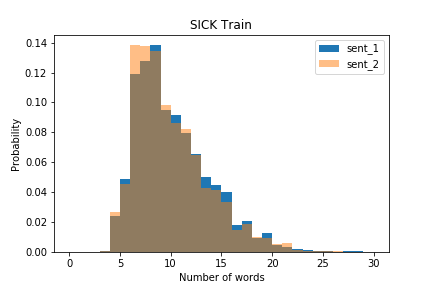
\includegraphics[width=\textwidth]{figures/semantic_textual_similarity/introduction/sick_train_words.png}
		\caption{Normalised distribution of word count in SICK training set}
		\label{fig:sick_train_words}
	\end{subfigure}%
	\begin{subfigure}[b]{.5\textwidth}
		\centering
		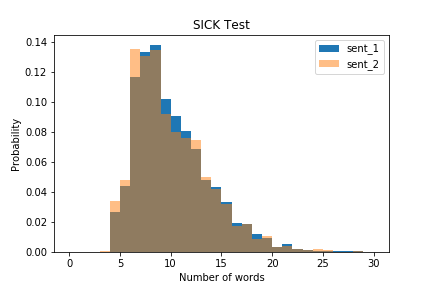
\includegraphics[width=\textwidth]{figures/semantic_textual_similarity/introduction/sick_test_words.png}
		\caption{Normalised distribution of word count in SICK test set}
		\label{fig:sick_test_words}
	\end{subfigure}
	\caption[Normalised distribution of word count in SICK training and SICK test sets.]{Normalised distribution of word count in SICK training and SICK test sets. \textit{Number of words} indicates the word count and \textit{Probability} shows the total probability of a sentence with that word count appearing in the dataset.}
	\label{fig:sick_words}
\end{figure}


\begin{table*}
	\centering
	\begin{tabular}{l|cc|cc}
		\hline
		Measure   & \multicolumn{2}{c|}{SICK Train} & \multicolumn{2}{c}{SICK Test} \\
		\hline
		\multicolumn{1}{l|}{} & \textbf{Sent$\_$1} & \textbf{Sent$\_$2} & \textbf{Sent$\_$1} & \textbf{Sent$\_$2} \\
		\textit{Word Count Mean} & 9.73 & 9.52 & 9.69 & 9.53  \\
		\textit{Word Count STD} & 3.66 & 3.70 & 3.69 & 3.65  \\
		\textit{Word Count MAX} & 28 & 32 & 28 & 30  \\
		\textit{Word Count MIN} & 3 & 3 & 3 & 3  \\
		\hline
	\end{tabular}
	\caption[Word count stats in SICK]{Word count stats in SICK training and SICK test sets. \textit{STD} indicates the standard deviation and the other acronyms indicate the common meaning }
	\label{table:sick_sts}
\end{table*}



The common consensus in STS is that when two sentences share a large number of words, the relatedness of those two sentences should be higher. In fact, in early feature-based approaches of calculating semantic textual similarity, the number of overlapping words between the two sentences was a common feature \autocite{vilarino-etal-2014-buap,  gupta-etal-2014-uow, lynum-etal-2014-ntnu, chavez-etal-2014-umcc}. Systems such as \textcite{vilarino-etal-2014-buap} and \textcite{lynum-etal-2014-ntnu}, directly use the number of words common in two sentences as a feature, while systems like \textcite{gupta-etal-2014-uow} and \textcite{chavez-etal-2014-umcc} use Jaccard Similarity Coefficient as a feature, which is a measurement based on word overlap. To observe whether the number of common words from the two sentences has a relationship on the relatedness, we draw a violin plot\footnote{Violin plots are similar to box plots, except that they also show the probability density of the data at different values, usually smoothed by a kernel density estimator.} for each relatedness score bins with word share in Figure \ref{fig:sick_word_share}.


\begin{figure}
	\captionsetup[subfigure]{justification=centering}
	\centering
	\begin{subfigure}[b]{.5\textwidth}
		\centering
		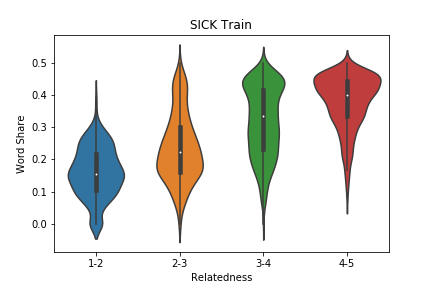
\includegraphics[width=\textwidth]{figures/semantic_textual_similarity/introduction/sick_train_word_share.png}
		\caption{Word share against relatedness bins in SICK training set}
		\label{fig:sick_train_word_share}
	\end{subfigure}%
	\begin{subfigure}[b]{.5\textwidth}
		\centering
		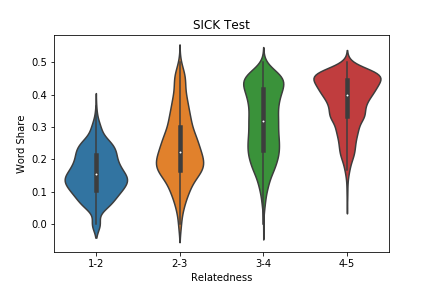
\includegraphics[width=\textwidth]{figures/semantic_textual_similarity/introduction/sick_test_word_share.png}
		\caption{Word share against relatedness bins in SICK test set}
		\label{fig:sick_test_word_share}
	\end{subfigure}
	\caption[Word share against relatedness bins in SICK training and SICK test sets.]{Word share against relatedness bins in SICK training and SICK test sets. \textit{Word Share} indicates the ratio between number of common words in the two sentences to total number of words in the two sentences against each \textit{Relatedness} bins}
	\label{fig:sick_word_share}
\end{figure}



In figure \ref{fig:sick_word_share}, it is clear that sentence pairs with a higher relatedness tend to have a high word share. However, it should be noted that, in the "2-3" relatedness score bin, there are some sentence pairs with a high word share. The most common example for such a case would be when \emph{sentence 2} is the complete negation of the \emph{sentence 1} \autocite{marelli-etal-2014-semeval}. In such cases, the two sentences share a large portion of the words, and one sentence has the \textit{"not"} word that gives a completely opposite meaning compared to the other sentence. Similarly "4-5" relatedness score bin has some sentence pairs with a low word share. Those sentence pairs do not contain the same words but have synonyms or paraphrases that result in the same overall meaning \autocite{marelli-etal-2014-semeval}. Therefore, the STS methods that focus on word share as a feature will not perform well in the SICK dataset \autocite{ranasinghe-etal-2019-enhancing}. 

A clear strength in the SICK dataset is that the training set and the test set reflect similar properties with regards to sentence length, relatedness distribution etc. Therefore, a machine learning model properly trained on the SICK training set should also give good results from the SICK test set \autocite{marelli-etal-2014-semeval}.  


 \item \textbf{STS 2017 English Dataset}\footnote{The STS 2017 English Dataset is available to download at \url{http://ixa2.si.ehu.es/stswiki/}} The second English STS dataset we used to experiment with in this thesis is the STS 2017 English Dataset, which was employed in \textit{SemEval-2017 Task 1: Semantic Textual Similarity Multilingual and Cross-lingual Focused Evaluation}, which is the most recent STS task in SemEval \autocite{cer-etal-2017-semeval}. As the training data for the competition, participants were encouraged to make use of all existing data sets from prior STS evaluations, including all previously released trial, training and evaluation data from SemEval 2012 - 2016 \autocite{agirre-etal-2012-semeval,agirre-etal-2013-sem,agirre-etal-2014-semeval,agirre-etal-2015-semeval,agirre-etal-2016-semeval}. Once combined, we had 8277 sentence pairs for training. More information about the datasets used to build the training set is available in Table \ref{tab:englishdata_info}.
 
 
 
 \begin{table}[ht!]
 	\centering
 	\begin{tabular}{c|c|c|l}
 		\hline
 		\multicolumn{1}{c|}{\textbf{Year}} & 
 		\multicolumn{1}{c|}{\textbf{Dataset}} & 
 		\multicolumn{1}{c|}{\textbf{Pairs}} & 
 		\multicolumn{1}{c}{\textbf{Source}} \\
 		\hline
 		 \multirow{5}{*}{\makecell{2012 \\ \autocite{agirre-etal-2012-semeval}}} & MSRpar & 1500 & newswire \\
 		 & MSRvid & 1500 & videos \\
 		 & OnWN & 750 & glosses \\
 		 & SMTnews & 750 & WMT eval. \\
 		 & SMTeuroparl & 750 & WMT eval. \\
 		\hline
 		 \multirow{4}{*}{\makecell{2013 \\ \autocite{agirre-etal-2013-sem}}} & HDL & 750 & newswire \\
 		 & FNWN & 189 & glosses \\
 		 & OnWN & 561 & glosses \\
 		 & SMT & 750 & MT eval. \\
 		\hline
 		 \multirow{6}{*}{\makecell{2014 \\ \autocite{agirre-etal-2014-semeval}}} & HDL & 750 & newswire headlines \\
 		 & OnWN & 750 & glosses \\
 		 & Deft-forum & 450 & forum posts \\
 		 & Deft-news & 300 & news summary \\
 		 & Images & 750 & image descriptions \\
 		 & Tweet-news & 750 & tweet-news pairs \\
 		\hline
 		 \multirow{5}{*}{\makecell{2015 \\ \autocite{agirre-etal-2015-semeval}} } & HDL & 750 & newswire headlines \\
 		 & Images & 750 & image descriptions \\
 		& Ans.-student & 750 & student answers \\
 		 & Ans.-forum & 375 & Q\&A forum answers \\
 		 & Belief & 375 & committed belief \\
 		\hline
 		 \multirow{5}{*}{\makecell{2016 \\ \autocite{agirre-etal-2016-semeval} }} & HDL & 249 & newswire headlines \\
 		 & Plagiarism & 230 & short-answer plag. \\
 		& post-editing & 244 & MT postedits \\
 		 & Ans.-Ans. & 254 & Q\&A forum answers \\
 		 & Quest.-Quest. & 209 & Q\&A forum questions \\
 		\hline
 		\makecell{2017 \\ \autocite{cer-etal-2017-semeval}} & Trial & 23 & Mixed STS 2016 \\
 		\hline
 	\end{tabular}
 	\caption[Information about English STS 2017 training set]{Information about the datasets used to build the English STS 2017 training set. The \textbf{Year} column shows the year of the SemEval competition that the dataset was released. The \textbf{Dataset} column expresses the acronym used describe a dataset in that year. The \textbf{Pairs} column shows the number of sentence pairs in that particular dataset and the \textbf{Source} column shows the source of the sentence pairs. }
 	\label{tab:englishdata_info}
 \end{table}

On the other hand, a fresh test set of 250 sentence pairs was provided by SemEval-2017 STS Task organisers \autocite{cer-etal-2017-semeval}. The Stanford Natural Language Inference (SNLI) corpus \autocite{bowman-etal-2015-large} was the primary data source for this test set. Similarly to the SICK dataset, each pair in the STS 2017 English Test set has been annotated to mark the degree to which the two sentence meanings are related (on a 5-point scale). The ratings have been collected through crowdsourcing on Amazon Mechanical Turk\footnote{Amazon Mechanical Turk is a crowdsourcing website for businesses to hire remotely located \textit{crowd workers} to perform discrete on-demand tasks. It is available at \url{https://www.mturk.com/}}. Five annotations have been collected per pair, and the gold score has been computed for each pair as the average of the five ratings assigned by the annotators. However, unlike the SICK dataset, the organisers have a clear explanation for the score ranges. Table \ref{tab:sts2017data} shows some example sentence pairs from the dataset with the gold labels and their explanations. Similarly to the SICK dataset, the machine learning models require predicting a value between 0-5 to reflect the similarity of the given sentence pair \autocite{cer-etal-2017-semeval}.

 
   \begin{table}[ht!]
 	\centering 	
 	\begin{tabular}{l|c} 
 		\hline
 		\multicolumn{1}{c|}{\textbf{Sentence Pair}} & 
 		\multicolumn{1}{c}{\textbf{Relatedness}}  \\
 		\hline
 		\makecell[l]
 		{\textit{The two sentences are completely equivalent}  \\ \textit{as they mean the same thing.} \\
 			1. The bird is bathing in the sink. \\ 
 			2. Birdie is washing itself in the water basin.} & 5  \\
 		\hline
 		\makecell[l]
 		{\textit{The two sentences are mostly equivalent, but}  \\ \textit{some unimportant details differ.} \\
 			1. Two boys on a couch are playing video games. \\ 
 			2. Two boys are playing a video game.} & 4  \\
 		\hline
 		\makecell[l]
 		{\textit{The two sentences are roughly equivalent, but }  \\ \textit{some important information differs/missing.} \\
 			1. John said he is considered a witness but not \\ a suspect. \\ 
 			2. “He is not a suspect anymore.” John said.} & 3  \\
 		\hline
 		\makecell[l]
 		{\textit{The two sentences are not equivalent, but share } \\
 			\textit{some details.} \\
 			1. They flew out of the nest in groups. \\ 
 			2. They flew into the nest together.} & 2  \\
 		\hline
 		\makecell[l]
 		{\textit{The two sentences are not equivalent, but are } \\
 			\textit{on the same topic.} \\
 			1. The woman is playing the violin. \\ 
 			2. The young lady enjoys listening to the guitar.} & 1  \\
 		\hline
 		\makecell[l]
 		{\textit{The two sentences are completely dissimilar} \\
 			1. The black dog is running through the snow. \\ 
 			2. A race car driver is driving his car through \\ the mud.} & 0  \\
 		\hline
 	
 	\end{tabular}
 	\caption[Example sentence pairs from the STS2017 English dataset]{Example sentence pairs from the STS2017 English dataset with their gold relatedness scores (on a 5-point rating scale) and explanations. The \textbf{Sentence Pair} column shows the two sentences and the \textbf{Relatedness} column denotes the annotated relatedness score.}
 	\label{tab:sts2017data}
 \end{table} 

\begin{figure}
	\captionsetup[subfigure]{justification=centering}
	\centering
	\begin{subfigure}[b]{.5\textwidth}
		\centering
		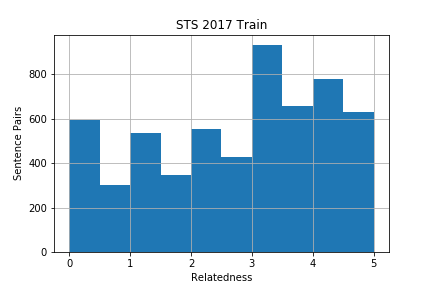
\includegraphics[width=\textwidth]{figures/semantic_textual_similarity/introduction/sts_train.png}
		\caption{Relatedness distribution of \\ STS 2017 training test}
		\label{fig:sts_train_relatedness}
	\end{subfigure}%
	\begin{subfigure}[b]{.5\textwidth}
		\centering
		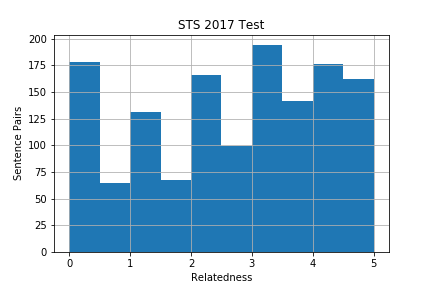
\includegraphics[width=\textwidth]{figures/semantic_textual_similarity/introduction/sts_test.png}
		\caption{Relatedness distribution of \\ STS 2017 test set}
		\label{fig:sts_test_relatedness}
	\end{subfigure}
	\caption[Relatedness distribution of STS 2017 training and STS 2017 test sets]{Relatedness distribution of STS 2017 training and STS 2017 test sets. \textit{Sentence Pairs} shows the number of sentence pairs that a certain \textit{Relatedness bin} has.}
	\label{fig:sts_relatedness}
\end{figure}

As with the SICK dataset, we conduct an exploratory data analysis on the STS2017 dataset. Figure \ref{fig:sts_relatedness} shows the relatedness distribution, and Figure \ref{fig:sts_words} shows the normalised distribution of word count for \emph{sentence 1} and \emph{sentence 2} in the STS 2017 training and test sets. Most of these statistics are similar to the SICK dataset. One notable change is the maximum word count in the STS 2017 training dataset, which is 57 in \emph{sentence 1} and 48 in \emph{sentence 2} according to Table \ref{table:sts_2017_sts} while both SICK datasets' and STS 2017 test set's maximum word count is limited to 30. We believe that the reason for this is the STS training dataset is composed from many sources including news articles that can have lengthy sentences. However, the STS algorithm should be able to properly handle this imbalanced nature between the STS2017 training and test sets \autocite{cer-etal-2017-semeval}. 

\begin{figure}
	\captionsetup[subfigure]{justification=centering}
	\centering
	\begin{subfigure}[b]{.5\textwidth}
		\centering
		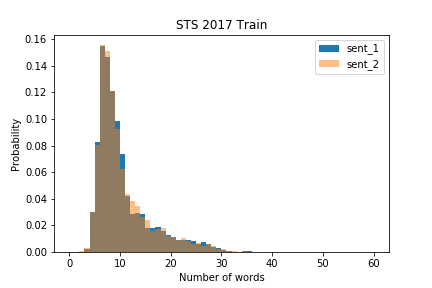
\includegraphics[width=\textwidth]{figures/semantic_textual_similarity/introduction/sts_2017_train_words.png}
		\caption{Normalised distribution of word count in STS 2017 training set}
		\label{fig:sts_train_words}
	\end{subfigure}%
	\begin{subfigure}[b]{.5\textwidth}
		\centering
		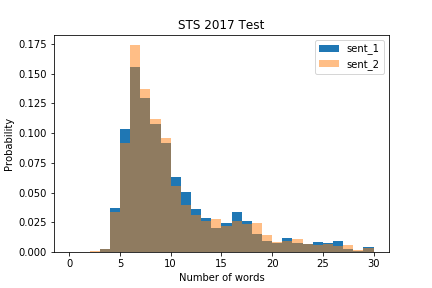
\includegraphics[width=\textwidth]{figures/semantic_textual_similarity/introduction/sts_2017_test_words.png}
		\caption{Normalised distribution of word count in STS 2017 test set}
		\label{fig:sts_test_words}
	\end{subfigure}
	\caption[Normalised distribution of word count in STS 2017 training and STS 2017 test sets.]{Normalised distribution of word count in STS 2017 training and STS 2017 test sets. \textit{Number of words} indicates the word count and \textit{Probability} shows the total probability of a sentence with that word count appearing in the dataset.}
	\label{fig:sts_words}
\end{figure}



In Figure \ref{fig:sts_word_share}, we draw a violin plot for each relatedness score bin with word share. We can see that generally, a higher word share leads to higher relatedness, but still, there can be sentence pairs that contradict this, which is similar to the observation we had with the SICK dataset. 


\begin{table*}
	\centering
	\begin{tabular}{l|cc|cc}
		\hline
		Measure   & \multicolumn{2}{c|}{STS 2017 Train} & \multicolumn{2}{c}{STS 2017 Test} \\
		\hline
		\multicolumn{1}{l|}{} & \textbf{Sent$\_$1} & \textbf{Sent$\_$2} & \textbf{Sent$\_$1} & \textbf{Sent$\_$2} \\
		\textit{Word Count Mean} & 10.01 & 9.94 & 9.83 & 9.80  \\
		\textit{Word Count STD} & 5.52 & 5.36 & 5.14 & 5.14  \\
		\textit{Word Count MAX} & 57 & 48 & 30 & 30  \\
		\textit{Word Count MIN} & 3 & 2 & 3 & 2  \\
		\hline
	\end{tabular}
	\caption[Word count stats in STS 2017]{Word count stats in STS 2017 training and STS 2017 test sets. \textit{STD} indicates the standard deviation and the other acronyms indicate the common meaning }
	\label{table:sts_2017_sts}
\end{table*}

Since the statistics of SICK and STS 2017 datasets are similar, one dataset can be used to augment the training data in the other dataset or perform transfer learning, which can lead to better results as neural networks perform better with more data \autocite{wang-etal-2020-evaluating,info:doi/10.2196/23086}. We hope to experiment on this with supervised machine learning models in Chapters \ref{cha:sts_siamese_neural_networks} and \ref{cha:sts_transformers}.

\begin{figure}
	\captionsetup[subfigure]{justification=centering}
	\centering
	\begin{subfigure}[b]{.5\textwidth}
		\centering
		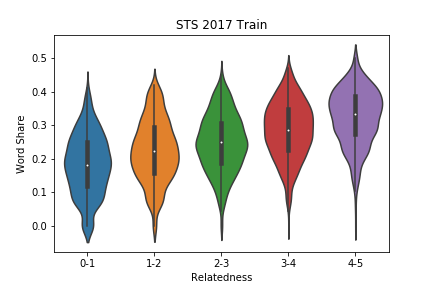
\includegraphics[width=\textwidth]{figures/semantic_textual_similarity/introduction/sts_2017_train_word_share.png}
		\caption{Word share against relatedness bins in STS 2017 training set}
		\label{fig:sts_train_word_share}
	\end{subfigure}%
	\begin{subfigure}[b]{.5\textwidth}
		\centering
		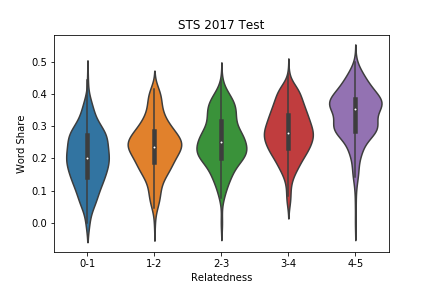
\includegraphics[width=\textwidth]{figures/semantic_textual_similarity/introduction/sts_2017_test_word_share.png}
		\caption{Word share against relatedness bins in STS 2017 test set}
		\label{fig:sts_test_word_share}
	\end{subfigure}
	\caption[Word share against relatedness bins in STS 2017 training and STS 2017 test sets.]{Word share against relatedness bins in STS 2017 training and STS 2017 test sets. \textit{Word Share} indicates the ratio between number of common words in the two sentences to total number of words in the two sentences against each \textit{Relatedness} bins}
	\label{fig:sts_word_share}
\end{figure}


 \begin{table}[ht!]
	\centering 	
	\begin{tabular}{l|c} 
		\hline
		\multicolumn{1}{c|}{\textbf{Question Pair}} & 
		\multicolumn{1}{c}{\textbf{\detokenize{is-duplicate}}}  \\
		\hline
		\makecell[l]
		{	1. What are natural numbers? \\ 
			2. What is a least natural number?} & 0  \\
		\hline
		\makecell[l]
		{	1. Which Pizzas are most popularly ordered \\ in Dominos menu? \\ 
			2. How many calories does a Dominos Pizza have?} & 0  \\
		\hline
		\makecell[l]
		{   1. How do you start a bakery? \\ 
			2. How can one start a bakery business?} & 1  \\
		\hline
		\makecell[l]
		{	1. Should I learn Python or Java first? \\ 
			2. If I had to choose between learning \\ Java and Python what should I choose \\ to learn first?} & 1  \\
		\hline
		
	\end{tabular}
	\caption[Example question pairs from the Quora Question Pairs dataset]{Example question  pairs from the Quora Question Pairs dataset with their gold \detokenize{is-duplicate} value. \textbf{Question Pair} column shows the two questions and \textbf{is-duplicated} column denotes whether it is a duplicated pair or not.}
	\label{tab:quoradata}
\end{table}  


 \item \textbf{Quora Question Pairs}\footnote{The Quora Question Pairs Dataset is available to download at \url{http://qim.fs.quoracdn.net/quora_duplicate_questions.tsv}} The Quora Question Pairs dataset is a big dataset that was first released for a Kaggle Competition\footnote{Kaggle is an online community of data scientists and machine learning practitioners that hosts machine learning competitions. The Quora Question Pairs competition is available on \url{https://www.kaggle.com/c/quora-question-pairs}}. Quora is a question-and-answer website where internet users ask, answer, follow, and edit questions, either factually or in the form of opinions. If a particularly new question has been asked before, users merge the new question to the original question flagging it as a duplicate. The organisers used this functionality to create the dataset and did not use a separate annotation process. Their original sampling method has returned an imbalanced dataset with many more true examples of duplicate pairs than non-duplicates. Therefore, the organisers have supplemented the dataset with negative examples. One source of negative examples has been pairs of \textit{related question} which belongs to similar topics but are not truly equivalent semantically.  
 

 \begin{figure}
 	\captionsetup[subfigure]{justification=centering}
 	\centering
 	\begin{subfigure}[b]{.5\textwidth}
 		\centering
 		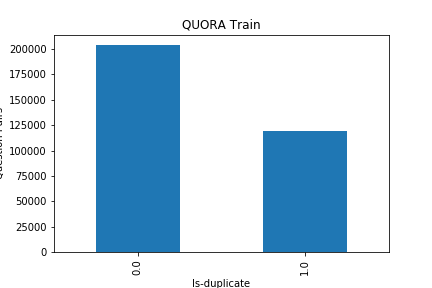
\includegraphics[width=\textwidth]{figures/semantic_textual_similarity/introduction/quora_train.png}
 		\caption{Is-duplicate distribution of \\ QUORA training set}
 		\label{fig:quora_train_is_duplicate}
 	\end{subfigure}%
 	\begin{subfigure}[b]{.5\textwidth}
 		\centering
 		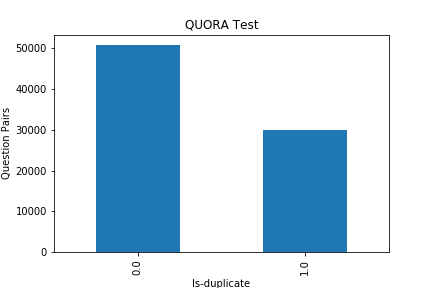
\includegraphics[width=\textwidth]{figures/semantic_textual_similarity/introduction/quora_test.png}
 		\caption{Is-duplicate distribution of \\ QUORA test set}
 		\label{fig:quora_test_is_duplicate}
 	\end{subfigure}
 	\caption[Is-duplicate distribution of QUORA training and QUORA test sets]{Is-duplicate distribution of QUORA training and QUORA test sets. \textit{Sentence Pairs} shows the number of sentence pairs that a certain \textit{Is-duplicate} has.}
 	\label{fig:quora_is_duplicate}
 \end{figure}
   

The dataset has 400,000 question pairs, and we used a 4:1 split to separate it into a training set and a test set, resulting in 320,000 questions pairs in the training set and  80,000 sentence pairs in the test set. The machine learning models need to predict a continuous value between 0 and 1 that reflects whether it is a duplicate question pair or not. 1 indicates that a particular question pair is a duplicate, and 0 means it is not a duplicate. 


This dataset is different from the previous datasets as it is not artificially created and uses day-to-day language. Since it has more than 300,000 training instances, deep learning systems will benefit more from using this dataset. 


\begin{figure}
	\captionsetup[subfigure]{justification=centering}
	\centering
	\begin{subfigure}[b]{.5\textwidth}
		\centering
		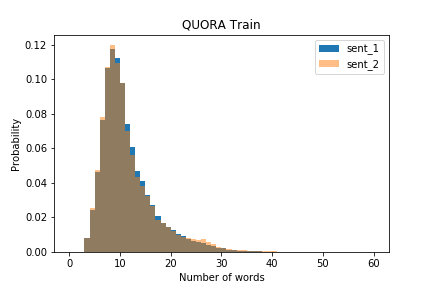
\includegraphics[width=\textwidth]{figures/semantic_textual_similarity/introduction/quora_train_words.png}
		\caption{Normalised distribution of word count in QUORA training set}
		\label{fig:quora_train_words}
	\end{subfigure}%
	\begin{subfigure}[b]{.5\textwidth}
		\centering
		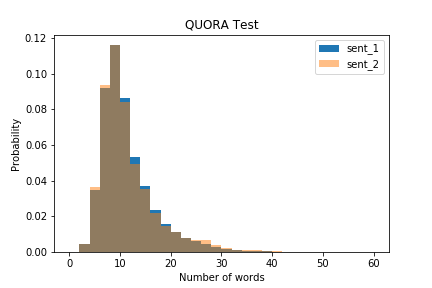
\includegraphics[width=\textwidth]{figures/semantic_textual_similarity/introduction/quora_test_words.png}
		\caption{Normalised distribution of word count in QUORA test set}
		\label{fig:quora_test_words}
	\end{subfigure}
	\caption[Normalised distribution of word count in QUORA training and QUORA test sets.]{Normalised distribution of word count in QUORA training and QUORA test sets. \textit{Number of words} indicates the word count and \textit{Probability} shows the total probability of a sentence with that word count appearing in the dataset.}
	\label{fig:quora_words}
\end{figure}

In Figure \ref{fig:quora_is_duplicate} we show the distribution of the two classes in the QUORA dataset. The dataset seems to have more non-duplicate question pairs than duplicate sentence pairs, similar to the real-world scenario. According to the word count distribution in Figure \ref{fig:quora_words} and word count statistics in Table \ref{table:quora_sts}, it is clear that the QUORA datasets contain longer texts than the SICK and STS 2017 datasets. Therefore, the QUORA dataset should be able to test the machine learning models' ability to handle lengthy texts properly. 

\begin{figure}
	\captionsetup[subfigure]{justification=centering}
	\centering
	\begin{subfigure}[b]{.5\textwidth}
		\centering
		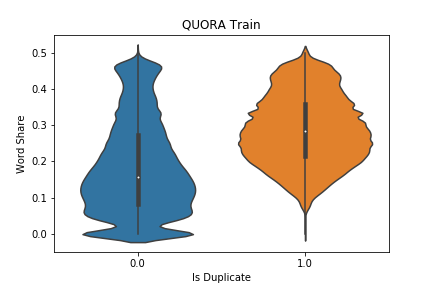
\includegraphics[width=\textwidth]{figures/semantic_textual_similarity/introduction/quora_train_word_share.png}
		\caption{Word share against is-relatedness value in QUORA training set}
		\label{fig:quora_train_word_share}
	\end{subfigure}%
	\begin{subfigure}[b]{.5\textwidth}
		\centering
		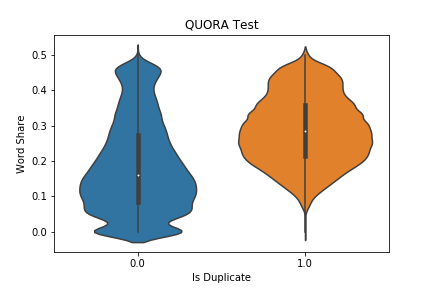
\includegraphics[width=\textwidth]{figures/semantic_textual_similarity/introduction/quora_test_word_share.png}
		\caption{Word share against is-relatedness value in QUORA test set}
		\label{fig:quora_test_word_share}
	\end{subfigure}
	\caption[Word share against Is-duplicate values in QUORA training and QUORA test sets.]{Word share against Is-duplicate values in QUORA training and QUORA test sets. \textit{Word Share} indicates the ratio between number of common words in the two sentences to total number of words in the two sentences against each \textit{Is-duplicate}}
	\label{fig:quora_word_share}
\end{figure}

In Figure \ref{fig:quora_word_share} we show a violin plot for each \textit{"is-duplicate"} value with word share. We can see that duplicate questions have a high word share. However, it should be noted that there are non-duplicate question pairs that still have a high word share. This shows that determining STS is not a trivial task. 

According to statistics provided by the Director of Product Management at Quora on 17 September 2018, over 100 million people visit Quora every month, which raises the problem of different users asking similar questions with the same intent but with different wording \autocite{8967103}. Multiple questions with the same intent can cause seekers to spend more time finding the best answer to their question and make writers feel they need to answer multiple versions of the same question. Therefore, identifying duplicate questions will make finding high-quality answers to questions easier, resulting in an improved experience for Quora writers, seekers, and readers.


\begin{table*}
	\centering
	\begin{tabular}{l|cc|cc}
		\hline
		Measure   & \multicolumn{2}{c|}{QUORA Train} & \multicolumn{2}{c}{QUORA Test} \\
		\hline
		\multicolumn{1}{l|}{} & \textbf{Ques$\_$1} & \textbf{Ques$\_$2} & \textbf{Ques$\_$1} & \textbf{Ques$\_$2} \\
		\textit{Word Count Mean} & 10.95 & 11.20 & 10.92 & 11.14  \\
		\textit{Word Count STD} & 5.44 & 6.31 & 5.40 & 6.31  \\
		\textit{Word Count MAX} & 125 & 237 & 73 & 237  \\
		\textit{Word Count MIN} & 1 & 1 & 1 & 1  \\
		\hline
	\end{tabular}
	\caption[Word count stats in QUORA]{Word count stats in QUORA training and QUORA test sets.\textit{STD} indicates the standard deviation and the other acronyms indicate the common meaning }
	\label{table:quora_sts}
\end{table*}
 
  


\end{enumerate}

\subsection{Datasets on Other Languages}
One of the main requirements of our research was to build an STS method without depending on the language. Therefore throughout our study, we worked on several datasets from different languages. Those non-English datasets are described below. 

\begin{table}[ht!]
	\centering 	
	\begin{tabular}{l|c} 
		\hline
		\multicolumn{1}{c|}{\textbf{Sentence Pair}} & 
		\multicolumn{1}{c}{\textbf{\detokenize{Similarity}}}  \\
		\hline
		\makecell[l]
		{	1. \< أحدهم يقلي لحما.  > \\ \textit{Someone is frying meat.}\ \\ 
			2.  \< أحدهم يعزف البيانو.  > \\ \  \textit{Someone plays the piano.} } & 0.250
		\\
		\hline
		\makecell[l]
		{	1. \< أمرأة تظيف المكونات في الإناء.  > \\ \textit{
				A woman cleaning ingredients in the bowl.}\ \\ 
			2.  \< إمرأة تكسر ثلاثة بيضات في الإناء. > \\ \  \textit{
				A woman breaks three eggs in a bowl.} } & 1.750
		\\
		\hline
		\makecell[l]
		{	1. \< طفلة تعزف القيثارة.  > \\ \textit{A Child is playing harp.}\ \\ 
			2.  \< رجل يعزف القيثارة . > \\ \  \textit{A man plays the harp.} } & 2.250
		\\
		\hline
		\makecell[l]
		{	1. \< المرأة تقطع البصل الأخضر.  > \\ \textit{The woman chops green onions.}\ \\ 
			2.  \< إمرأة تقشر بصلة. > \\ \  \textit{A woman peeling an onion.} } & 3.250
		\\
		\hline
		\makecell[l]
		{	1. \< الأيل قفز فوق السياج. > \\ \textit{The deer jumped over the fence.}\ \\ 
			2.  \< أيل يقفز فوق سياج الإعصار. > \\ \  \textit{Deer Jumps Over Hurricane Fence} } & 4.800
		\\
		\hline
		
	\end{tabular}
	\caption[Example question pairs from the Arabic STS dataset]{Example question  pairs from the Arabic STS dataset. The \textbf{Sentence Pair} column shows the two sentences. We also included their translations in the table. The translations were done by a native Arabic speaker. The \textbf{Similarity} column indicates the annotated similarity of the two sentences.}
	\label{tab:arabicdata}
\end{table}  

  
\begin{enumerate}
\item{ \textbf{Arabic STS Dataset \footnote{The Arabic STS dataset can be downloaded at \url{http://alt.qcri.org/semeval2017/task1/index.php?id=data-and-tools}}}} The Arabic STS dataset we selected was also used for the Arabic STS subtask in \textit{SemEval 2017 Task 1: Semantic Textual Similarity Multilingual and Cross-lingual Focused Evaluation} \autocite{cer-etal-2017-semeval}. Unlike for English, there was no data from previous SemEval competitions available since this was the first time an Arabic STS task was organised in SemEval. More information about the extracted sentences will be shown in Table \ref{tab:arabicdata_info}. 

\begin{table}[ht!]
	\centering
	\begin{tabular}{c|c|l}
		\hline
		\multicolumn{1}{c|}{\textbf{Dataset}} & 
		\multicolumn{1}{c|}{\textbf{Pairs}} & 
		\multicolumn{1}{c}{\textbf{Source}} \\
		\hline
		Trial & 23 & Mixed STS 2016 \\
		MSRpar  & 510 & newswire \\
		MSRvid  & 368 & videos \\
		SMTeuroparl  & 203 & WMT eval. \\
		\hline
	\end{tabular}
	\caption[Information about Arabic STS training set]{Information about the datasets used to build the Arabic STS training set. The \textbf{Dataset} column expresses the acronym used describe the dataset. The \textbf{Pairs} column shows the number of sentence pairs in that particular dataset and \textbf{Source} column shows the source of the sentence pairs. }
	\label{tab:arabicdata_info}
\end{table} 

\begin{figure}
	\captionsetup[subfigure]{justification=centering}
	\centering
	\begin{subfigure}[b]{.5\textwidth}
		\centering
		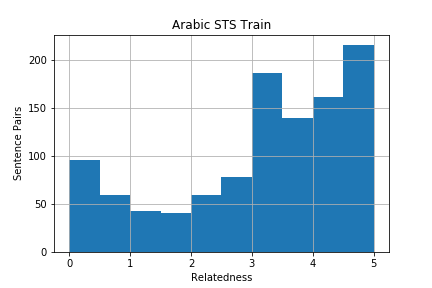
\includegraphics[width=\textwidth]{figures/semantic_textual_similarity/introduction/sts_arabic_train.png}
		\caption{Relatedness distribution of \\ Arabic STS  training set}
		\label{fig:arabic_train_relatedness}
	\end{subfigure}%
	\begin{subfigure}[b]{.5\textwidth}
		\centering
		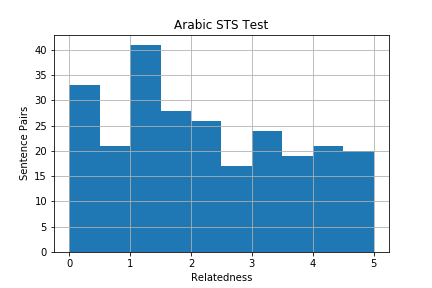
\includegraphics[width=\textwidth]{figures/semantic_textual_similarity/introduction/sts_arabic_test.png}
		\caption{Relatedness distribution of \\ Arabic STS  test set}
		\label{fig:arabic_test_relatedness}
	\end{subfigure}
	\caption[Relatedness distribution of Arabic STS training and Arabic STS test sets]{Relatedness distribution of Arabic STS training and Arabic STS test sest. \textit{Sentence Pairs} shows the number of sentence pairs that a certain \textit{Relatedness bin} has.}
	\label{fig:arabic_sts_relatedness}
\end{figure} 



A subset of the English STS 2017 dataset has been selected and human translated into Arabic to prepare the annotated instances. Sentences have been translated independently from their pairs. The Arabic translations have been provided by native Arabic speakers with strong English skills at Carnegie Mellon University in Qatar. Translators have been given an English sentence and its Arabic machine translations where they have performed post-editing to correct errors. STS labels have then been transferred to the translated pairs. Therefore, the annotation guidelines and the template are similar to those for the English STS 2017 dataset. 1103 sentence pairs were available for training, and 250 sentence pairs were available in the test set. Table \ref{tab:arabicdata} shows a few pairs of sentences with their similarity scores. The machine learning models require a value to be predicted between 0-5, which reflects the similarity of a given Arabic sentence pair. 



Similarly to the English STS datasets, we also analysed the Arabic STS dataset considering the same set of properties. As can be seen in Figure \ref{fig:arabic_sts_relatedness}, the relatedness distribution is different in the training and test sets. In the training set, there are many sentences with high relatedness scores compared to low relatedness scores. On the other hand,  there are many sentences with low relatedness scores compared to the high relatedness scores in the test set.


\begin{figure}
	\captionsetup[subfigure]{justification=centering}
	\centering
	\begin{subfigure}[b]{.5\textwidth}
		\centering
		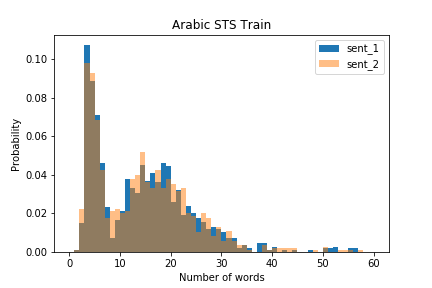
\includegraphics[width=\textwidth]{figures/semantic_textual_similarity/introduction/arabic_sts_train_words.png}
		\caption{Normalised distribution of word count in Arabic STS training set}
		\label{fig:arabic_sts_train_words}
	\end{subfigure}%
	\begin{subfigure}[b]{.5\textwidth}
		\centering
		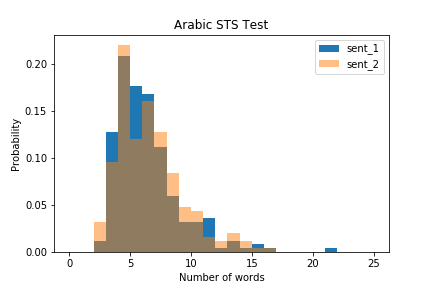
\includegraphics[width=\textwidth]{figures/semantic_textual_similarity/introduction/arabic_sts_test_words.png}
		\caption{Normalised distribution of word count in Arabic STS test set}
		\label{fig:arabic_sts_test_words}
	\end{subfigure}
	\caption[Normalised distribution of word count in Arabic STS training and Arabic STS test sets.]{Normalised distribution of word count in Arabic STS training and Arabic STS test sets. \textit{Number of words} indicates the word count and \textit{Probability} shows the total probability of a sentence with that word count appearing in the dataset.}
	\label{fig:arabic_sts_words}
\end{figure}

Word count distribution in the training and test sets of the Arabic dataset is also different. As shown in Figure \ref{fig:arabic_sts_words} the sentences in the training set are longer than the sentences in the test set. This is further confirmed by the statistics in Table \ref{table:arabic_sts}. The average word count in the training set is 31, while this is 9 in the test set. With these observations, we can conclude that the Arabic training set and test are different with regards to several properties. This nature of the dataset may be a challenge for ML systems.

\begin{figure}
	\captionsetup[subfigure]{justification=centering}
	\centering
	\begin{subfigure}[b]{.5\textwidth}
		\centering
		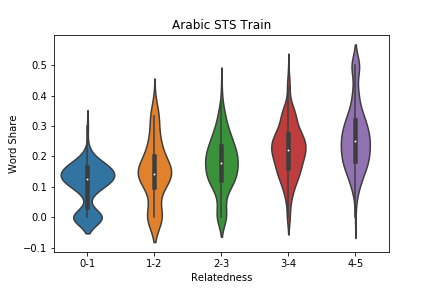
\includegraphics[width=\textwidth]{figures/semantic_textual_similarity/introduction/arabic_sts_train_word_share.png}
		\caption{Word share against relatedness bins in Arabic STS training set}
		\label{fig:arabic_sts_train_word_share}
	\end{subfigure}%
	\begin{subfigure}[b]{.5\textwidth}
		\centering
		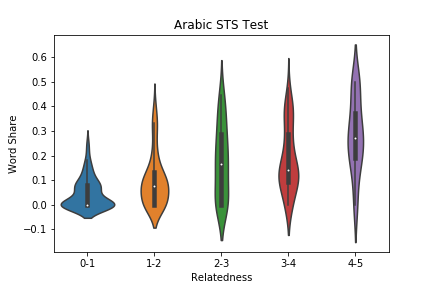
\includegraphics[width=\textwidth]{figures/semantic_textual_similarity/introduction/arabic_sts_test_word_share.png}
		\caption{Word share against relatedness bins in Arabic STS test set}
		\label{fig:arabic_sts_test_word_share}
	\end{subfigure}
	\caption[Word share against relatedness bins in Arabic STS training and Arabic STS test sets.]{Word share against relatedness bins in Arabic STS training and Spanish STS test sets. \textit{Word Share} indicates the ratio between number of common words in the two sentences to total number of words in the two sentences against each \textit{Relatedness} bins}
	\label{fig:arabic_sts_word_share}
\end{figure}

In Figure \ref{fig:arabic_sts_word_share}, we draw a violin plot for each relatedness bin with word share. The higher word share generally leads to higher similarity. However, there are sentence pairs that contradict this theory. This observation is similar to the results from the English datasets. 


\begin{table*}
	\centering
	\begin{tabular}{l|cc|cc}
		\hline
		Measure   & \multicolumn{2}{c|}{Arabic STS Train} & \multicolumn{2}{c}{Arabic STS Test} \\
		\hline
		\multicolumn{1}{l|}{} & \textbf{Sent$\_$1} & \textbf{Sent$\_$2} & \textbf{Sent$\_$1} & \textbf{Sent$\_$2} \\
		\textit{Word Count Mean} & 31.23 & 31.02 & 9.03 & 9.34  \\
		\textit{Word Count STD} & 12.15 & 12.37 & 3.66 & 3.74  \\
		\textit{Word Count MAX} & 90 & 90 & 22 & 24  \\
		\textit{Word Count MIN} & 5 & 1 & 3 & 3  \\
		\hline
	\end{tabular}
	\caption[Word count stats in Arabic STS]{Word count stats in Arabic STS training and Arabic STS test sets.\textit{STD} indicates the standard deviation and the other acronyms indicate the common meaning }
	\label{table:arabic_sts}
\end{table*}	

\begin{table}[ht!]
	\centering
	\begin{tabular}{l|c}
		\hline
		\multicolumn{1}{c|}{\textbf{Sentence Pair}} & 
		\multicolumn{1}{c}{\textbf{Similarity}}  \\
		\hline
		\makecell[l]{1. Amás, los misioneros apunten que los númberos \\ d'infectaos puen ser shasta dos o hasta cuatro veces \\ más grandess que los oficiales. \\
			\textit{(Furthermore, missionaries point out that the numbers of } \\ \textit{infected can be up to two or up to four times larger than} \\ \textit{the official ones.)} \\ 
			2. Los cadáveres de personas fallecidas pueden ser hasta \\ diez veces más contagiosos que los infectados vivos. \\ 
			\textit{(The corpses of deceased people can be up to ten times } \\ \textit{more contagious than those infected alive.)}} & 0.6  \\
		\hline
		\makecell[l]{1. La policía abatió a un caníbal cuando devoraba a una  \\ mujer Matthew Williams, de 34 años, fue sorprendido en \\ la madrugada mordiendo el rostro de una joven a la que  \\ había invitado a su hotel. \\ 
			\textit{(Police killed a cannibal while devouring a woman Matthew } \\ \textit{Williams, 34, was caught early in the morning biting the} \\ \textit{ face of a young woman he had invited to his hotel.)} \\
			2. La policía de Gales del Sur mató a un caníbal cuando se \\ estaba comiendo la cara de una mujer de 22 años en la \\ habitación de un hotel. \\ 
			\textit{(South Wales police killed a cannibal when he was eating the } \\ \textit{face of a 22-year-old woman in a hotel room.)} } & 2  \\
		\hline
		\makecell[l]{1. Ollanta Humala se reúne mañana con el Papa Francisco. \\
			\textit{(Ollanta Humala meets tomorrow with Pope Francis.)} \\ 
			2. El Papa Francisco mantuvo hoy una audiencia privada \\ con el presidente Ollanta Humala, en el Vaticano. \\
			\textit{(Pope Francis held a private audience today with President} \\ \textit{Ollanta Humala, at the Vatican.)}} & 3  \\
		\hline               
	\end{tabular}
	\caption[Example sentence pairs from the Spanish STS dataset]{Example sentence pairs from the Spanish STS dataset. The \textbf{Sentence Pair} column shows the two sentences. We also included their translations in the table. The translations were done by a native Spanish speaker. The \textbf{Similarity} column indicates the annotated similarity of the two sentences. }
	\label{tab:spanishdata}
\end{table} 
	

\item{ \textbf{Spanish STS Dataset\footnote{The Spanish STS dataset can be downloaded at \url{http://alt.qcri.org/semeval2017/task1/index.php?id=data-and-tools}}}} - Spanish STS dataset that we used was employed for the Spanish STS subtask in \textit{SemEval 2017 Task 1: Semantic Textual Similarity Multilingual and Cross-lingual Focused Evaluation} \autocite{cer-etal-2017-semeval}. The training set has 1250 sentence pairs annotated with a relatedness score between 0 and 4. The training set combined several datasets from previous SemEval STS shared tasks \autocite{cer-etal-2017-semeval}. Table \ref{tab:spanishdata_info} shows more information about the training set. There were two sources for the test set - Spanish news and Spanish Wikipedia dump having 500 and 250 sentence pairs respectively \autocite{cer-etal-2017-semeval}. Both datasets were annotated with a relatedness score between 0 and 5. Table \ref{tab:spanishdata} shows several pairs of sentences with their similarity score. The machine learning models require to predict a value between 0-5, which reflects the similarity of the given Spanish sentence pair.


\begin{table}[ht!]
	\centering
	\begin{tabular}{c|c|c|l}
		\hline
		\multicolumn{1}{c|}{\textbf{Year}} & 
		\multicolumn{1}{c|}{\textbf{Dataset}} & 
		\multicolumn{1}{c|}{\textbf{Pairs}} & 
		\multicolumn{1}{c}{\textbf{Source}} \\
		\hline
		 \multirow{3}{*}{\makecell{2014 \\ \autocite{agirre-etal-2014-semeval}}} & Trial & 56 & NR \\
		 & Wiki  & 324 & Spanish Wikipedia \\
		 & News  & 480 & Newswire \\
		\hline
		\multirow{2}{*}{\makecell{2015 \\ \autocite{agirre-etal-2015-semeval} }} & Wiki & 251 & Spanish Wikipedia \\
		 & News & 500 & Newswire \\
		\hline
	\end{tabular}
	\caption[Information about Spanish STS training set]{Information about the datasets used to build the Spanish STS training set. The \textbf{Year} column shows the year of the SemEval competition that the dataset got released. The \textbf{Dataset} column expresses the acronym used describe a dataset in that year. The \textbf{Pairs} column shows the number of sentence pairs in that particular dataset and the \textbf{Source} shows the source of the sentence pairs. }
	\label{tab:spanishdata_info}
\end{table}


\begin{figure}
	\captionsetup[subfigure]{justification=centering}
	\centering
	\begin{subfigure}[b]{.5\textwidth}
		\centering
		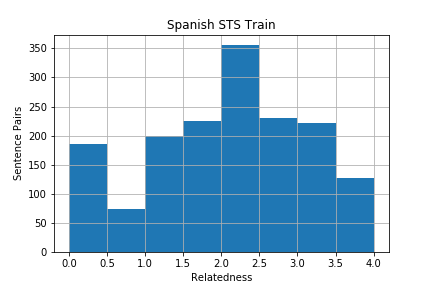
\includegraphics[width=\textwidth]{figures/semantic_textual_similarity/introduction/sts_spanish_train.png}
		\caption{Relatedness distribution of \\ Spanish STS  training test}
		\label{fig:spanish_train_relatedness}
	\end{subfigure}%
	\begin{subfigure}[b]{.5\textwidth}
		\centering
		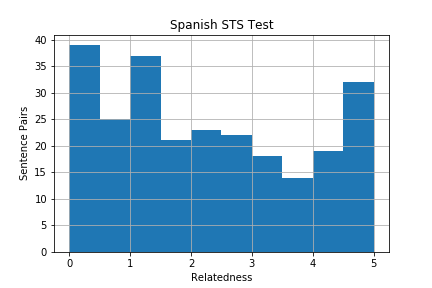
\includegraphics[width=\textwidth]{figures/semantic_textual_similarity/introduction/sts_spanish_test.png}
		\caption{Relatedness distribution of \\ Spanish STS  test set}
		\label{fig:spanish_test_relatedness}
	\end{subfigure}
	\caption[Relatedness distribution of Spanish STS training and Spanish STS test sets]{Relatedness distribution of Spanish STS training and Spanish STS test sets. \textit{Sentence Pairs} shows the number of sentence pairs that a certain \textit{Relatedness bin} has.}
	\label{fig:spanish_sts_relatedness}
\end{figure}


Similarly to the Arabic STS dataset, we analysed the Spanish STS dataset considering the same set of properties. A key challenge in the Spanish STS dataset too is that the test set is very different from the training set. As can be seen in Figure \ref{fig:spanish_sts_relatedness}, the training set has been annotated with relatedness scores 0-4 while the test set has been annotated with relatedness scores 0-5. Therefore, STS methods need to be developed to ensure that they can handle this situation. This can be observed as a weakness in this dataset, but at the same time, this property of the dataset can be exploited to measure the robustness of an STS system.

\begin{figure}
	\captionsetup[subfigure]{justification=centering}
	\centering
	\begin{subfigure}[b]{.5\textwidth}
		\centering
		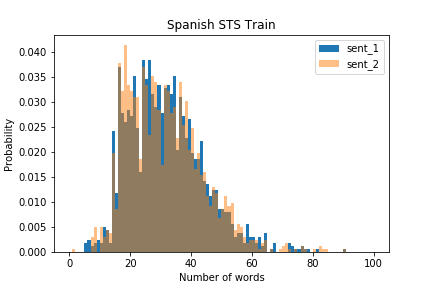
\includegraphics[width=\textwidth]{figures/semantic_textual_similarity/introduction/spanish_sts_train_words.png}
		\caption{Normalised distribution of word count in Spanish STS training set}
		\label{fig:spanish_sts_train_words}
	\end{subfigure}%
	\begin{subfigure}[b]{.5\textwidth}
		\centering
		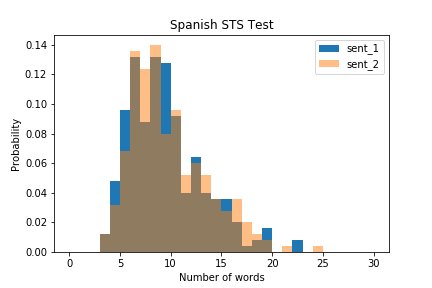
\includegraphics[width=\textwidth]{figures/semantic_textual_similarity/introduction/spanish_sts_test_words.png}
		\caption{Normalised distribution of word count in Spanish STS test set}
		\label{fig:spanish_sts_test_words}
	\end{subfigure}
	\caption[Normalised distribution of word count in Spanish STS training and Spanish STS test sets.]{Normalised distribution of word count in Spanish STS training and Spanish STS test sets. \textit{Number of words} indicates the word count and \textit{Probability} shows the total probability of a sentence with that word count appearing in the dataset.}
	\label{fig:spanish_sts_words}
\end{figure}

Furthermore, as shown in Figure \ref{fig:spanish_sts_words} and Table \ref{table:spanish_sts} sentence pairs in the test set are shorter in word length than the sentence pairs in the training set. Therefore, STS methods working on this dataset should also be able to properly handle that. This is similar to what we observed with the Arabic STS dataset.




\begin{figure}
	\captionsetup[subfigure]{justification=centering}
	\centering
	\begin{subfigure}[b]{.5\textwidth}
		\centering
		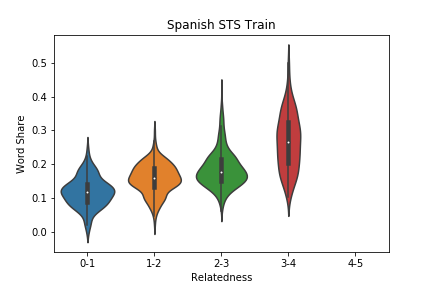
\includegraphics[width=\textwidth]{figures/semantic_textual_similarity/introduction/spanish_sts_train_word_share.png}
		\caption{Word share against relatedness bins in Spanish STS training set}
		\label{fig:spanish_sts_train_word_share}
	\end{subfigure}%
	\begin{subfigure}[b]{.5\textwidth}
		\centering
		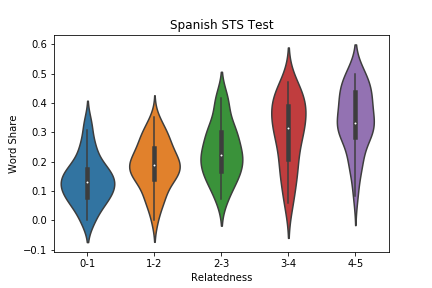
\includegraphics[width=\textwidth]{figures/semantic_textual_similarity/introduction/spanish_sts_test_word_share.png}
		\caption{Word share against relatedness bins in Spanish STS test set}
		\label{fig:spanish_sts_test_word_share}
	\end{subfigure}
	\caption[Word share against relatedness bins in Spanish STS training and STS 2017 test sets.]{Word share against relatedness bins in Spanish STS training and Spanish STS test sets. \textit{Word Share} indicates the ratio between number of common words in the two sentences to total number of words in the two sentences against each \textit{Relatedness} bins}
	\label{fig:spanish_sts_word_share}
\end{figure}

The violin plot between the word share against the relatedness bin in Spanish STS is similar to the previous datasets we analysed. As can be seen in Figure \ref{fig:spanish_sts_word_share}, a higher word share leads to a higher similarity, but some sentence pairs contradict this.


\begin{table*}
	\centering
	\begin{tabular}{l|cc|cc}
		\hline
		Measure   & \multicolumn{2}{c|}{Spanish STS Train} & \multicolumn{2}{c}{Spanish STS Test} \\
		\hline
		\multicolumn{1}{l|}{} & \textbf{Sent$\_$1} & \textbf{Sent$\_$2} & \textbf{Sent$\_$1} & \textbf{Sent$\_$2} \\
		\textit{Word Count Mean} & 31.23 & 31.02 & 9.03 & 9.34  \\
		\textit{Word Count STD} & 12.15 & 12.37 & 3.66 & 3.74  \\
		\textit{Word Count MAX} & 90 & 90 & 22 & 24  \\
		\textit{Word Count MIN} & 5 & 1 & 3 & 3  \\
		\hline
	\end{tabular}
	\caption[Word count stats in Spanish STS]{Word count stats in Spanish STS training and Spanish STS test sets.\textit{STD} indicates the standard deviation and the other acronyms indicate the common meaning }
	\label{table:spanish_sts}
\end{table*}

	
\end{enumerate}


\subsection{Datasets on Different Domains}
To experiment with how our STS methods can be adopted into different domains, we also used a dataset from a different discipline which we introduce in this section. 
\begin{enumerate}
	
	\item{ \textbf{Biomedical STS Dataset: BIOSSES}\footnote{Biomedical STS Dataset: BIOSSES  can be downloaded from \url{https://tabilab.cmpe.boun.edu.tr/BIOSSES/DataSet.html} }} - BIOSSES is the first and only benchmark dataset for biomedical sentence similarity estimation \autocite{10.1093/bioinformatics/btx238}. The dataset comprises of 100 sentence pairs, in which each sentence has been selected from the TAC (Text Analysis Conference) Biomedical Summarisation Track - training dataset containing articles from the biomedical domain \footnote{Biomedical Summarisation Track is a shared task organised in TAC 2014 - \url{https://tac.nist.gov/2014/BiomedSumm/}}. The sentence pairs have been evaluated by five different human experts that judged the similarity and gave scores ranging from 0 (no relation) to 4 (equivalent). The score range described was based on the guidelines of SemEval 2012 Task 6 on STS \autocite{agirre-etal-2012-semeval}. Besides the annotation instructions, example sentences from the biomedical literature have also been provided to the annotators for each similarity degree. To represent the similarity between two sentences, we took the average of the scores provided by the five human experts. Table \ref{tab:biomeddata} shows a few examples from the dataset. The machine learning models require to predict a value between 0-4, which reflects the similarity of the given biomedical sentence pair.
	

	
	\begin{table}[ht!]
		\centering
			\begin{tabular}{c|c}
				\hline
				\multicolumn{1}{c|}{\textbf{Sentence Pair}} & 
				\multicolumn{1}{c}{\textbf{Similarity}}  \\
				\hline
				\makecell[l]{1. It has recently been shown that Craf is essential \\ for Kras G12D-induced NSCLC. \\ 
					2. It has recently become evident that Craf is \\ essential for the onset of Kras-driven non-small \\ cell lung cancer.} & 4  \\
				\hline
				\makecell[l]{1. Up-regulation of miR-24 has been observed in \\ a number of cancers, including OSCC. \\ 
					2. In addition, miR-24 is one of the most abundant \\ miRNAs in cervical cancer cells, and is reportedly \\ up-regulated in solid stomach cancers. } & 3 \\
				\hline
				\makecell[l]{1. These cells (herein termed TLM-HMECs) are \\ immortal but do not proliferate in the absence of \\ extracellular matrix (ECM) \\  
					2. HMECs expressing hTERT and SV40 LT \\ (TLM-HMECs) were cultured in mammary epithelial \\ growth medium (MEGM, Lonza)  } & 1.4  \\
				\hline
				\makecell[l]{1.The up-regulation of miR-146a was also detected in \\ cervical cancer tissues.  \\ 
					2. Similarly to PLK1, Aurora-A activity is required \\ for the enrichment or localisation of multiple \\ centrosomal  factors which have roles in maturation, \\ including LATS2 and CDK5RAP2/Cnn.} & 0.2  \\
				\hline               
			\end{tabular}
		\caption[Example question pairs from the BIOSSES dataset]{Example question  pairs from the BIOSSES dataset. The \textbf{Sentence Pair} column shows the two sentences. The \textbf{Similarity} column indicates the averaged annotated similarity of the two sentences.}
		\label{tab:biomeddata}
	\end{table} 

The relatedness distribution is shown in Figure \ref{fig:biosses_relatedness}. It is similar to the relatedness distribution we saw in SICK and STS2017, where there were more sentences with high relatedness scores than low relatedness scores.

\begin{figure}
	\centering
	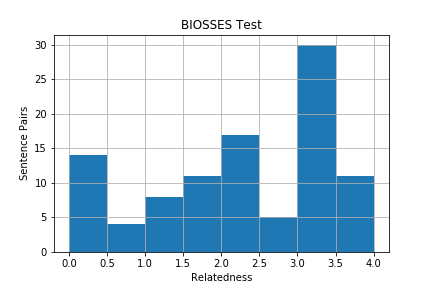
\includegraphics[width=0.8\textwidth]{figures/semantic_textual_similarity/introduction/biosses.png}
	\caption[Relatedness distribution of BIOSSES]{Relatedness distribution of BIOSSES. \textit{Sentence Pairs} shows the number of sentence pairs that a certain \textit{Relatedness bin} has.}
	\label{fig:biosses_relatedness}
\end{figure}

As shown in Figure \ref{fig:biosses_relatedness}, sentences in the BIOSSES dataset are longer than the sentences in the English datasets we mentioned before. The average length of a sentence in English datasets was below 15, while in the BIOSSES dataset, the average length is around 20. 

\begin{figure}
	\centering
	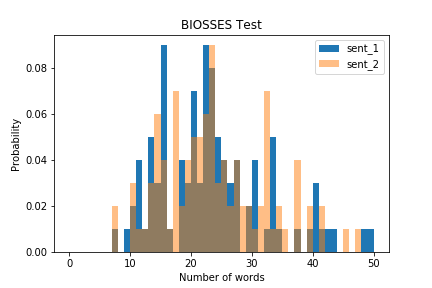
\includegraphics[width=0.8\textwidth]{figures/semantic_textual_similarity/introduction/biosses_words.png}
	\caption[Normalised distribution of word count in BIOSSES.]{Normalised distribution of word count in BIOSSES. \textit{Number of words} indicates the word count and \textit{Probability} shows the total probability of a sentence with that word count appearing in the dataset.}
	\label{fig:biosses_words}
\end{figure}

As we mentioned before, the BIOSSES dataset only has 100 sentence pairs. A dataset as small as this one can not be used to train a supervised ML method, requiring alternative approaches such as unsupervised methods and transfer learning techniques which we will be exploring in the following few chapters.

\begin{figure}
	\centering
	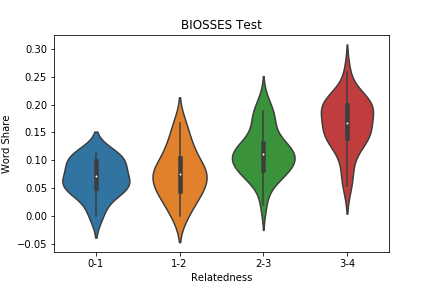
\includegraphics[width=0.8\textwidth]{figures/semantic_textual_similarity/introduction/biosses_word_share.png}
	\caption[Word share against relatedness bins in BIOSSES.]{Word share against relatedness bins in BIOSSES. \textit{Word Share} indicates the ratio between number of common words in the two sentences to total number of words in the two sentences against each \textit{Relatedness} bins}
	\label{fig:biosses_word_share}
\end{figure}


\end{enumerate}

\section{Evaluation Metrics}
\label{sec:sts_evaluation}
While training a machine learning model is a crucial step, how the model performs on unseen data is an equally important aspect that should be considered in every machine learning model. We need to know whether it actually works and, consequently, if we can trust its predictions. This is typically called as \textit{evaluation}. All of the datasets that we introduced in the previous section has what we call a \textit{test} set. The machine learning models need to provide their predictions for the test set, and the predictions will be evaluated against the gold values of the test set. 

There are three common evaluation metrics that are employed in Semantic Textual Similarity tasks, which we explain in this section. We will be using them to evaluate our models throughout the first part of our research. 

In the equations presented for each evaluation metrics, we represent the gold labels with $X$ and predictions with $Y$. Therefore, a gold label in the $i^{th}$ position will be represented by $X_i$ and the prediction in $i^{th}$ position will be represented by $Y_i$. 

\begin{enumerate}
	
	\item \textbf{Pearson's Correlation Coefficient} - Correlation is a technique for investigating the relationship between two quantitative, continuous variables. Pearson's correlation coefficient ($\rho$) measures the strength of the linear association between the two variables. A value of +1 is the total positive linear correlation between the variables, 0 is no linear correlation, and -1 is the total negative linear correlation. 
	
	Pearson's Correlation Coefficient is one of the most common evaluation metrics in STS shared tasks \autocite{marelli-etal-2014-semeval,agirre-etal-2012-semeval,agirre-etal-2013-sem,agirre-etal-2014-semeval,agirre-etal-2015-semeval,agirre-etal-2016-semeval}. A machine learning model with a Pearson's Correlation Coefficient close to 1 indicates that the predictions of that model and gold labels have a strong positive linear correlation. Therefore, it is a good model to predict STS. Pearson's Correlation Coefficient equation is shown in Equation \ref{equ:pearson} where $cov$  is the covariance, $\sigma_X$ is the standard deviation of $X$, and $\sigma_Y$ is the standard deviation of $Y$.
	
	\begin{equation}
	\label{equ:pearson}
	\rho = \frac{\text{cov}(X,Y)}{\sigma_X \sigma_Y}
	\end{equation}
	
	\item \textbf{Spearman's Correlation Coefficient} - Spearman's Correlation Coefficient ($\tau$) is another common evaluation metric in STS shared tasks \autocite{marelli-etal-2014-semeval,agirre-etal-2012-semeval,agirre-etal-2013-sem,agirre-etal-2014-semeval,agirre-etal-2015-semeval,agirre-etal-2016-semeval}. It assesses how well the relationship between two variables can be described using a monotonic function. A monotonic relationship is a relationship that does one of the following: 
	
	\begin{enumerate}
		\item as the value of one variable increases, so does the value of the other variable, \textit{or},
		\item as the value of one variable increases, the other variable value decreases.
	\end{enumerate}
	
	However, a monotonic relationship does not require a constant rate, whereas in a linear relationship, the rate of increase/decrease is constant. The fundamental difference between Pearson's correlation coefficient and Spearman's correlation coefficient is that Pearson's correlation coefficient only works with a linear relationship between the two variables, whereas the Spearman's correlation coefficient works with the monotonic relationships as well. Spearman's correlation coefficient is shown in Equation \ref{equ:spearman} where $D_i$ is the pairwise distances of the ranks of the variables $X_i$ and $Y_i$ and $n$ is the number of elements in $X$ or $Y$.   
	
	
	\begin{equation}
	\label{equ:spearman}
	\tau = 1- {\frac {6 \sum D_i^2}{n(n^2 - 1)}}
	\end{equation}
	
	In Spearman's correlation coefficient, a value of +1 is the total positive correlation between the variables, 0 is no correlation, and -1 is the total negative correlation. Therefore, similarly to Pearson's correlation coefficient, a machine learning model with a Spearman's Correlation Coefficient close to 1 indicates that the predictions of that model and gold labels have a strong positive correlation, and it is an excellent model to predict STS.
	
	\item \textbf{Root Mean Squared Error} - Both Pearson's Correlation Coefficient and Spearman's Correlation Coefficient only works when both gold labels($X$) and predictions ($Y$) are continuous. Therefore, for the datasets like Quora Question Pairs, where the gold labels are discrete values, Root Mean Squared Error (RMSE) is preferred for evaluation over Correlation Coefficient values. RMSE measures the distance between the gold labels and the predictions. RMSE equation is shown in Equation \ref{equ:rmse} where $n$ is the number of elements in $X$ or $Y$. 
	
	\begin{equation}
	\label{equ:rmse}
	RMSE = \sqrt{(\frac{1}{n})\sum_{i=1}^{n}(Y_{i} - X_{i})^{2}}
	\end{equation}

	In RMSE, a value close to 0 means that the error between the predictions and the gold labels are minimal. Therefore, a machine learning model with an RMSE value close to 1 indicates fewer errors and is an excellent model to predict STS.
	
\end{enumerate}

\section{Conclusion}
Calculating the STS is an important research area in NLP, which plays a vital role in many applications such as question answering, document summarisation, information retrieval and information extraction. Most of the early approaches were based on traditional machine learning and heavily involved in feature engineering. However, these approaches are difficult to be adapted for different languages and no longer provide competitive results. With the advances of word embeddings, and due to the success neural networks have achieved in other fields, most of the methods proposed in recent years rely on word vectors. These methods can be further categorised into supervised and unsupervised methods. Analysing STS methods belong to both of these categories would be beneficial to the community. Furthermore, exploring the ability of these methods to perform in a multilingual setting and a multi-domain setting would be a timely contribution to the NLP field. 

The introduction of competitive STS shared tasks has led to the development of standard datasets. We selected three recently released English STS datasets; SICK, STS2017 and Quora Question Pairs. They feature different characteristics. We exploratory analysed these datasets focussing on common properties such as the size of the dataset, sentence length, common number of words etc. Furthermore, we identified the specific properties of these datasets that would limit the performance of traditional STS methods like edit distance. For the multilingual experiments, we selected a Spanish and an Arabic dataset. Similarly to the English STS datasets, we exploratory analysed them for certain characteristics. For the multi-domain experiments, we chose a Biomedical STS Dataset. This dataset brings a key challenge to the STS methods as it does not have a separate training set. 

The STS shared tasks have further contributed to the development of evaluation measures in STS. In all of the datasets except Quora Question Pairs, Pearson Correlation and Spearman Correlation has been used to evaluate STS methods. In the Quora dataset, Root Mean Squared Error has been used to assess the methods. We followed the same evaluation measures in order to compare our methods with other systems submitted to the competition. 

In the next few chapters, we will be exploring different unsupervised and supervised STS methods. We will be evaluating them in English STS datasets, non-English STS datasets as well as out of domain STS datasets to investigate their adaptability in different environments.

   


